\documentclass[12pt]{article}
\usepackage[spanish]{babel}

%%%%%%%%%%%%%%%%%%%%%%%%%%%%%%%%%%
%%%%%%%%%%%%%%%%%%%%%%%%%%%%%   %%
%%        Datos Trabajo     %%  %%
%%%%%%%%%%%%%%%%%%%%%%%%%%%%%%%%%%
\newcommand{\titulo}[0]{Evidencia de aprendizaje:\\“Mi proyecto de investigación”\\\normalsize Parte 2}
\newcommand{\materia}[0]{Fundamentos de Investigación}
\newcommand{\grupo}[0]{BI-BFIN-2002-B2-013}
\newcommand{\unidad}[0]{Unidad 2}


%%%%%%%%%%%%%%%%%%%%%%%%%%%%%%%%%%
%%%%%%%%%%%%%%%%%%%%%%%%%%%%%%%%%%
\usepackage{amssymb}
\usepackage{enumerate}
\usepackage{mathtools}
\usepackage{multicol}
\usepackage{soul}

\usepackage{geometry}
	\geometry{margin=1.4in}
\usepackage{graphicx}
	\graphicspath{ {assets/} }
\usepackage{hyperref}
	\hypersetup{
			pdftex,
		        pdfauthor={bench},
		        pdftitle={\titulo},
		        pdfsubject={\materia},
		        pdfkeywords={\grupo, \unidad, UnADM},
		        pdfproducer={Latex with hyperref, Ubuntu},
		        pdfcreator={pdflatex, or other tool},
			colorlinks=true,
				linkcolor=[rgb]{0,0,0.4},
				urlcolor=cyan,
				filecolor=green,
				citecolor=blue}

%%%%%%%%%%%%%%%%%%%%%%%%%%%%%%%%%%
%%%%%%%%%%%%%%%%%%%%%%%%%%%%%%%%%%

\title{
	%
\includegraphics{../../../assets/logo-unadm} \\
	\ \\ Benjam\'in Rivera \\
	\bf{\titulo}\\\ \\}

\author{
	{\Huge Universidad Abierta y a Distancia de México} \\
	TSU en Biotecnolog\'ia \\
	\textit{Materia:} \materia \\
	\textit{Grupo:} \grupo \\
	\textit{Unidad:} \unidad \\
	\\
	\textit{Matricula:} ES202105994 }

\date{\textit{Fecha de entrega:} \today}



% Divulgación del campo de acción de la biotecnología mediante entes bioluminiscentes y fluorescentes
\newcommand{\tema}[0]{divulgación de campos de investigación de la biotecnología mediante entes bioluminiscentes y fluorescentes}
%%%%%%%%%%%%%%%%%%%%%%%%%%%%%
%%        Documento         %%
%%%%%%%%%%%%%%%%%%%%%%%%%%%%%%%
\begin{document}
\maketitle\newpage

\tableofcontents
\listoffigures
\newpage

\part*{\MakeUppercase{\tema}}



\section{Planteamiento}
	
	\par La Biotecnología no es, por el momento, la ingeniera mas conocida por el publico en general; a pesar de las grandes contribuciones que hace a la vida diaria, muchos desconocen el alcance que esta tiene. Esta falta de comprensión causa una mala imagen pública y complica el desarrollo de proyectos en esta área.
	\par Me interesa explorar el impacto de la difusión de áreas de acción en la percepción pública de la Biotecnología. Lo que, en formato de pregunta, puede ser escrito como
	\begin{quote}
		\textbf{\textit{¿Cómo afecta la difusión científica en la percepción pública de la Biotecnología con la población del estado de Guanajuato?}}
	\end{quote}
	  
	\noindent esta difusión esta pensada como la realización y explicación de experimentos con fines divulgativos. Específicamente se busca entender tres cosas:
	
	\begin{quote}
	\begin{enumerate}\it
			\item ¿Qué tan agradable son los experimentos con bioluminiscencia y fluorescencia en el público?
			\item ¿Qué experimentos tiene un mayor impacto\footnote{Tanto en retención del conocimiento, como en el impacto por los experimentos.}?
			\item ¿Qué clase de personas\footnote{Desde el punto de vista estadístico.} tienen la peor percepción respecto a la biotecnología? 

	\end{enumerate}
	\end{quote}






\newpage
\section{Objetivos}

	\par De manera que, tomando como preámbulo al planteamiento, el \textit{ objetivo principal } de este proyecto es	
	\begin{quote}

		\textbf{Desarrollar experimentos, no peligrosos, para la difusión de la Biotecnología y la medición de su impacto en la sociedad.}

	\end{quote}
	
	\noindent esto lo podemos trabajar en los siguientes \textit{ objetivos específicos }
	
	\begin{quote} \begin{enumerate} \it
		\item Determinar temas de interés para el publico en general que estén relacionados con la biotecnología. \label{obj: 1}
		\item Elaborar experimentos relacionados con los puntos anteriores, con un especial énfasis en aquellos que impliquen bioluminiscencia o fluorescencia. \label{obj: 2}
		\item Medir el impacto de los experimentos en distintas muestras de la población del estado de Guanajuato. \label{obj: 3}
	\end{enumerate} \end{quote}
	
	\noindent Podemos notar, a partir de la definición de los objetivos, que este proyecto es una investigación mixta. Dado que el objetivo \ref{obj: 1} requiere de datos cuantitativos y cualitativos; el objetivo \ref{obj: 2} trata de procesar información mixta y el objetivo \ref{obj: 3} trabajaría con información cuantitativa.






	
\section{Justificación}


	\par "Hoy no se discute la importancia que para la sociedad tienen la ciencia y la tecnología"\cite{CC}, o al menos de las disciplinas más famosas. El problema es que aún nos cuesta a entender a todos el alcance de todas estas y, por lo tanto, su impacto.	
	\par Tampoco es desconocido que la desinformación causa problemas y mitos que suelen perjudicar al desarrollo en general. La Biotecnología es una de las disciplinas que ha caído en un hoyo de desinformación; al ser una disciplina relativamente reciente, su pronta incorporación la ha llevado a un limbo en donde el público en general no sabe específicamente lo que es; al estar entre la investigación genética, el trabajo con biometeriales y el desarrollo de biotecnologías, no cualquiera puede comprender con facilidad lo que hace y el gran impacto que tiene en la vida cotidiana.
	\par El que el público en general no comprenda el campo de acción de esta disciplina, ocasiona que la imagen pública de esta sea negativa. Esto lleva a que tengamos artículos como \cite{filos} y \cite{mTransgenicos} que luego son tomados por medios sensacionalistas y publicados al mundo sin contexto alguno. Todo esto causa que se reduzcan los apoyos de financiamiento, recursos para la investigación en estas áreas.

	\par El uso de la divulgación como herramienta para cambio de percepción no es nuevo, solo por poner un ejemplo esta \cite{utilidad congresos}, donde se estudia la utilidad de los congresos como medio de difusión científica; o \cite{olimpiadas}, donde se estudia el impacto que eventos como las olimpiadas científicas tienen en los estudiantes.
	\par A pesar de que la biotecnología ya tiene estudios al respecto, estos deben ser replicados por cada zona geográfica\footnote{E incluso periódicamente}, esto por la naturalidad cambiante del ser humano. Existe un estudio que se realizó en el territorio español \cite{bio en espania} en el cual se platica de que, como ya he tratado de introducir en esta parte, la población en general siente temor acerca de la biotecnología principalmente por desconocimiento.
	\par Los experimentos se enfocaran a que el público entienda, hasta cierto punto, los procesos que se siguen durante la investigación. Además de mostrar que, cuando se trabaja con ética profesional y siguiendo los protocolos y regulaciones adecuadas, la biotecnología tiene un mayor impacto positivo que negativo. 
	\par El tener una especial atención en los experimentos con cosas que brillen\footnote{Fluorescentes y Bioluminiscentes} es para atraer rápidamente la atención de los mas chicos y que vayan jalando a los más grandes, por eso es necesario tener explicaciones de los experimentos para varios niveles. E incluso sería bueno usar nuevas tecnologías para aumentar la diversidad de opciones para comunicar; como se menciona en \cite{vr}.
	\par Este proyecto parte de una conclusión similar a la que se llego en \cite{biot mexico}. A pesar de que la percepción de la biotecnología en México es similar a la de otras regiones del mundo, de temor por desconocimiento, desde el aspecto científico y político se conocen bien todos los aspectos en donde los beneficios de la biotecnología son notables.







\newpage
\section{Marco Teórico}

	\par De manera que, aquí buscaremos la forma de sistematizar, definir y comprender el tema principal de esta investigación. Para esto definiremos que la hipótesis de este proyecto como sigue
	\begin{quote}\bf
		El uso de experimentos como herramienta de concientización y difusión de conceptos puede apoyar al entendimiento y aceptación social de los mismos.
	\end{quote}
	
	\noindent de manera que eso es lo que queremos justificar y sistematizar en esta sección.
	\ \\ \
	\par Los esfuerzos de distintas universidades,  como \cite{UG}, \cite{UdG}, \cite{unam}, para hacer constante divulgación, de estudios como \cite{utilidad congresos} y \cite{CC}, y de esfuerzos como los que se llevan a cabo en eventos como la olimpiada que son estudiados en \cite{olimpiadas}; nos permite poder hacer un poco de \textit{trampa} y empezar directamente con que la hipótesis \textit{la divulgación apoya directamente al mejoramiento da la imagen social de la ciencia}, ya que estos ya recorrieron, fundamentaron, y lo siguen haciendo constantemente, este camino.
	\par Partiendo de esto lo próximo que es bueno notar, a partir del estado del arte, es la percepción de que se tiene actualmente. En función de las conclusiones a las que se llegó en los artículos \cite{bio en espania}, \cite{a}, \cite{biot mexico} y \cite{b} podemos notar que no es la mejor; aunque por otro lado, como podemos apreciar en \cite{biohacker}, \cite{usos}, ademas de los avances mostrados en artículos como  \cite{genetica en colombia} y \cite{socializacion}, muestran claramente que los beneficios que esta disciplina emergente puede ofrecer a la sociedad en general son vastos.
	\par Como ventaja para este proyecto, este no es el primer esfuerzo que se hace para tratar de apoyar la imagen de la biotecnología. Una tendencia interesante es la popularización y simplificación para volver más accesibles ciertos experimentos; ejemplo de esto son \cite{kits} y \cite{kits2}, que buscan crear opciones accesibles para tener material básico de laboratorio para hacer experimentos básicos de biotecnología; esto tiene un pequeño inconveniente, a pesar de que todo este material esta pensado para ser \textit{más accesible}, los costos siguen sin ser para cualquier persona. 
	\par Una manera de solucionar la desventaja del punto anterior es usar alternativas de visualización e interacción como se propone en \cite{vr} y \cite{vr2}; que a pesar de que aún no son métodos que se apliquen en esta disciplina, no hay ninguna limitante teórica que lo limite.









%%%%%%%%%%%%%%%%%%%%%%%%%%%%%%%%
%%         Bibliografia        %%
%%%%%%%%%%%%%%%%%%%%%%%%%%%%%%%%%%
\newpage
\addcontentsline{toc}{section}{Referencias}
\begin{thebibliography}{X}
	\bibitem[Gordillo et al, 2003]{CC} Gordillo, M. M., \& Osorio, C. (2003). \textit{ Educar para participar en ciencia y tecnología. Un proyecto para la difusión de la cultura científica }. Revista Iberoamericana de Educación, 32(1), 8.
	
	\bibitem[Maliandi, 2003]{filos} Maliandi, R. (2003). \textit{ Ética y biotecnología: cuestión de principios. Agora Philosophica. } Revista Marplatense de Filosofía, 5(6), 34-56.
	
	\bibitem[Mandianes, 2009]{mTransgenicos} Mandianes, M. (2009, January). \textit{ La ruptura. El miedo moderno a la comida. In Humanismo para el siglo XXI: Propuestas para el Congreso Internacional" Humanismo para el siglo XXI" } (Vol. 31, p. 227). Universidad de Deusto.
	
	\bibitem[Ruiz et al, 2007]{utilidad congresos}Ruiz Santos, C., \& Meroño Cerdán, A. L. (2007). \textit{ Utilidad de los congresos científicos en la difusión del conocimiento: percepción del investigador español en Economía de la Empresa }.
	
	\bibitem[Vargas et al, 2012]{olimpiadas}Vargas, S. C., \& Chaves, J. P. (2012). \textit{ Construcción de la dimensión cognitiva de alfabetización científica en el estudiantado, a través de las Olimpiadas Costarricenses de Ciencias Biológicas }. Revista electrónica educare, 16(2), 217-236.
	
	\bibitem[Font, 2003]{bio en espania}Font, M. C. (2003). \textit{ Avances de la biotecnología y su percepción por la población española}. Boletín Económico de ICE, (2781).
	
	\bibitem[Monsalve et al, 2004]{a} Monsalve, I., de la Montaña Cámara, M., \& Cuesta, P. (2004). \textit{ Percepción de la biotecnología por los médicos de familia }. Quark, 51-56.
	
	\bibitem[Biosca, 2004]{b} Biosca, D. (2004). \textit{ Percepción pública de la Biotecnología }. Quark, 8-9.
	
	\bibitem[Aerni, 2001]{biot mexico}Aerni, P. (2001). \textit{ La percepción pública de la biotecnología agrícola en México }. Cambridge, MA: Science Technology and Innovation Policy (STI) Research Report. Harvard University.
	
	\bibitem[Campos et al, 2020]{vr} Campos Soto, M. N., Navas-Parejo, M. R., \& Moreno Guerrero, A. J. (2020). \textit{ Realidad virtual y motivación en el contexto educativo: Estudio bibliométrico de los últimos veinte años de Scopus }. ALTERIDAD. Revista de Educación, 15(1), 47-60.
	
	\bibitem[Biotecnia, 2020]{Biotecnia} Biotecnia$-$Home Page. (s/f). Recuperado el 18 de octubre de 2020, de \url{http://www.scielo.org.mx/scielo.php?script=sci_serial&pid=1665-1456&lng=es&nrm=iso}

	\bibitem[Vodafone, 2020]{biohacker} Biotecnología: “hackear” bacterias para fabricar cualquier cosa. (s/f). Recuperado el 18 de octubre de 2020, de \url{https://www.youtube.com/watch?v=cyst4EDDwAk}
	
	\bibitem[Cancino, 2020]{genetica en colombia} Cancino Escalante, G., Chaparro Giraldo, A., Cancino Escalante, G., \& Chaparro Giraldo, A. (2020). Status of scientific research and the Access to genetic resources by Colombian research groups. Revista Colombiana de Biotecnología, 22(1), 70-8. \url{https://doi.org/10.15446/rev.colomb.biote.v22n1.79451}

	\bibitem[UdG]{UdG} Diálogos sobre educación. Temas actuales en investigación educativa—Home Page. (s/f). Recuperado el 18 de octubre de 2020, de \url{http://www.scielo.org.mx/scielo.php?script=sci_serial&pid=2007-2171&lng=es&nrm=iso}
	
	\bibitem[UNAM]{unam} Divulgación de la Ciencia, UNAM. (s/f). Divulgación de la Ciencia, UNAM. Recuperado el 18 de octubre de 2020, de \url{http://www.dgdc.unam.mx/}
	
	\bibitem[UNAM FQ]{educacion quimica} Educación química—Home Page. (s/f). Recuperado el 18 de octubre de 2020, de \url{http://www.scielo.org.mx/scielo.php?script=sci_serial&pid=0187-893X&lng=es&nrm=iso}
	
	\bibitem[Discovery Channel, 2020]{usos} El uso de la biotecnología para combatir las epidemias $|$ Mosquito $|$ Discovery Latinoamérica. (s/f). Recuperado el 18 de octubre de 2020, de \url{https://www.youtube.com/watch?v=SLQFRUXNLQM}
	
	\bibitem [Garcia, 2019]{socializacion} García Jiménez, E., Gatica Arias, A.M., Solano Campos, F., \& Abdelnour Esquivel, A. (2019). Experiencia práctica: Socialización de conceptos, aplicaciones y beneficios de la biotecnología en Costa Rica experience: socializing the concepts, applications and benefits of biotechnology in Costa Rica. Revista de Biología Tropical, 67(2 SUPL), S26-S35. \url{https://doi.org/10.15517/rbt.v67i2SUPL.37201}
	
	\bibitem[Youtube, 2020]{kits} Kits educativos para hacer prácticas de biotecnología. (s/f). Recuperado el 18 de octubre de 2020, de \url{https://www.youtube.com/watch?v=Tillxa6fa3s}
	
	\bibitem[Massarani, 2020]{engajamiento} Massarani, L., Leal, T., \& Waltz, I. (2020). O debate sobre vacinas em redes sociais: Uma análise exploratória dos links com maior engajamento. Cadernos de Saúde Pública, 36, e00148319. \url{https://doi.org/10.1590/0102-311x00148319}
	
	\bibitem[Rodriguez, 2016]{}  Rodríguez Villafuerte, M., \& Rodríguez Villafuerte, M. (2016). Instituto de Física-UNAM. Mundo nano. Revista interdisciplinaria en nanociencias y nanotecnología, 9(16), 57-76. \url{https://doi.org/10.22201/ceiich.24485691e.2016.16.56901}
	
	\bibitem[eUGreka]{UG} Universidad de Guanajuato $|$ eUGreka Tu conecte con la ciencia. (s/f). Recuperado el 18 de octubre de 2020, de \url{https://www.ugto.mx/eugreka/}
	
	\bibitem[Alvarado, 2010]{} Alvarado Rodríguez, M. E., \& Flores Camacho, F. (2010). Percepciones y supuestos sobre la enseñanza de la ciencia: Las concepciones de los investigadores universitarios. Perfiles educativos, 32(128), 10-26. Recuperado en 28 de octubre de 2020, de \url{http://www.scielo.org.mx/scielo.php?script=sci_arttext&pid=S0185-26982010000200002&lng=es&tlng=es}
	
	\bibitem[Viñas, 2020]{kits2} Viñas, J., López, M. R., Pavisic, C. I., \& Riccioni, L. (2020). Biomaking": cómo hacer un laboratorio de biotecnología" low cost. Alambique: Didáctica de las ciencias experimentales, (99), 35-42.
	
	\bibitem[Argueta, 2020]{vr2} Argueta, M. L. A. A. Uso de Realidad Virtual para la formación de arquitectos. Accesible en \url{https://static1.squarespace.com/static/55564587e4b0d1d3fb1eda6b/t/5f73a1a4c489d610c40478f9/1601413561306/Tomo+01+-+Diseminaci%C3%B3n+de+resultados+de+investigaci%C3%B3n+universitaria+-+Tabasco+2020.pdf}


\end{thebibliography}


%%%%%%%%%%%%%%%%%%%%%%%%%%%%
%%        Apendices        %%
%%%%%%%%%%%%%%%%%%%%%%%%%%%%%%
\appendix\newpage
\section{Infografía}
\begin{figure}[h]
	\centering
		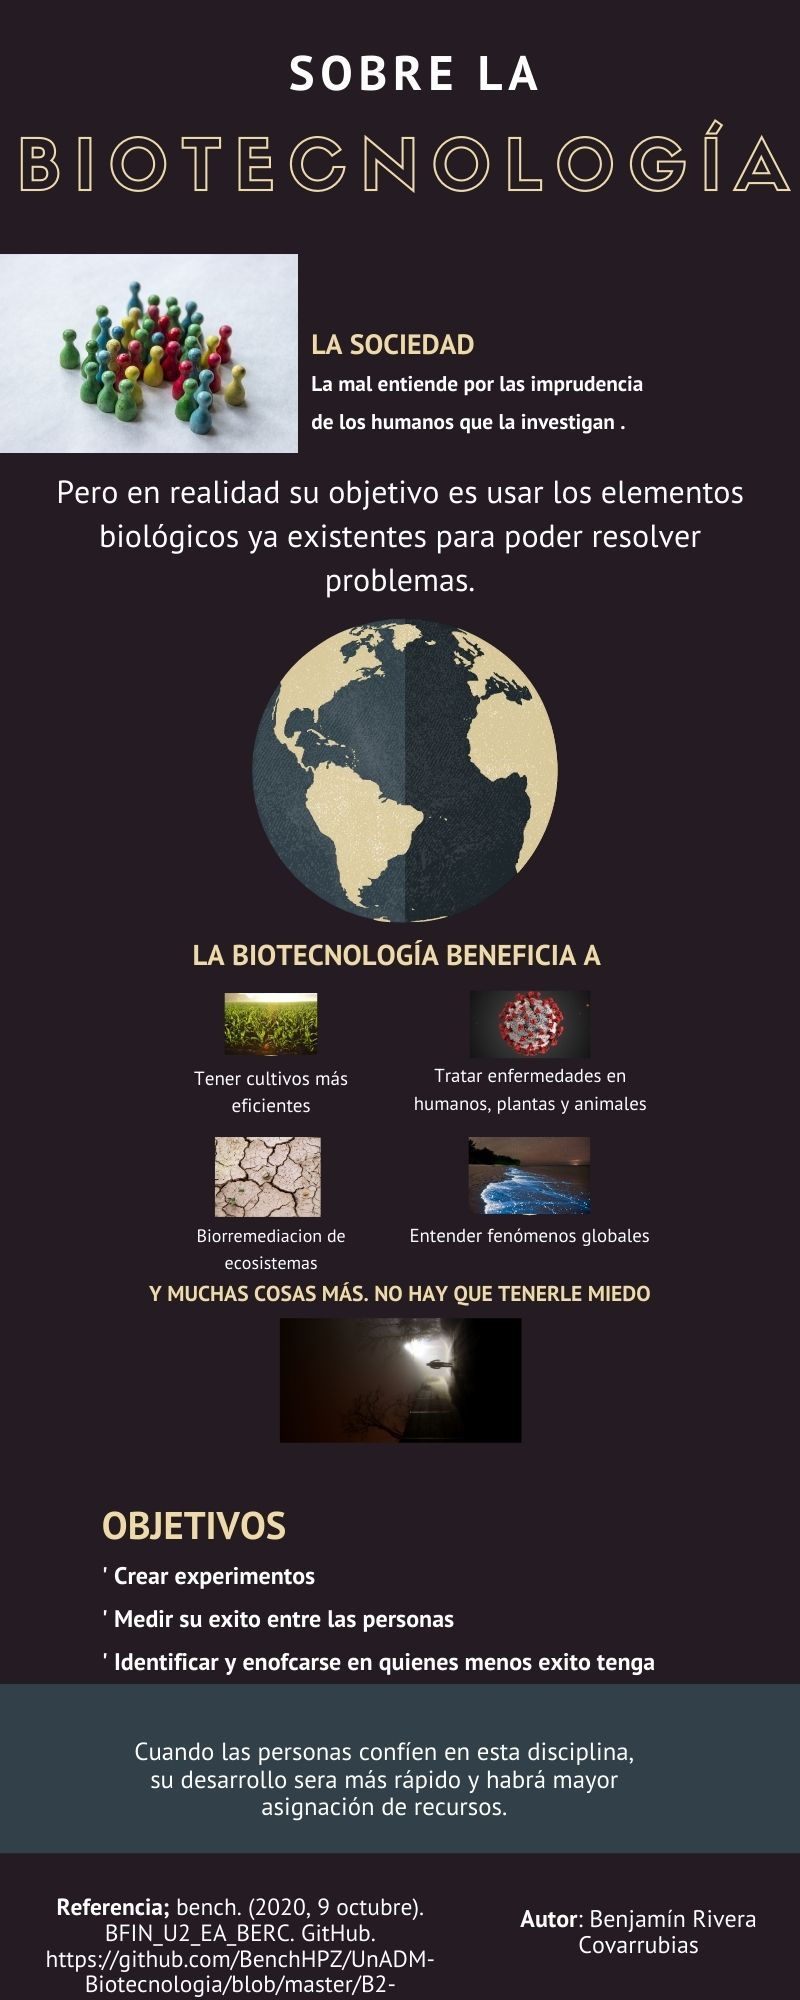
\includegraphics[height=0.7\textheight]{infografia_biotecnologia.jpg}
	\caption{Infografia de la \tema.}
	\label{fig: }
\end{figure}



\end{document}